\section{性能模型：先算上界，再谈优化}
\label{sec:perf}

性能模型的价值不在于精确预测，而在于给出\emph{可被违反就说明有 bug 的上界}。本节介绍面试中最常用的五个模型：
roofline、Amdahl/Gustafson、work--span、Little 定律以及 I/O 复杂度下界。

\subsection{Roofline 与算术强度}

Williams 等人提出的 roofline 模型~\cite{williams2009roofline} 把一个 kernel 抽象为两个数：浮点运算量 $F$ 与
它在某一级存储（通常是 DRAM/HBM）上搬运的字节数 $B$。定义算术强度 $I=F/B$（FLOP/byte），则在计算与访存可重叠时
\begin{equation}
t \ge \max\!\left(\frac{F}{P_{\text{peak}}},\ \frac{B}{\mathrm{BW}}\right),\qquad
P_{\text{attain}} = \min(P_{\text{peak}},\ I\cdot \mathrm{BW}).
\label{eq:roofline}
\end{equation}
两项相等的点 $I^\ast = P_{\text{peak}}/\mathrm{BW}$ 称为拐点（ridge point）：$I<I^\ast$ 的 kernel 受访存限制（memory-bound），
$I>I^\ast$ 的受算力限制（compute-bound）。以本文统一使用的参数（附录表~\ref{tab:hw}）计算，H100 SXM 的稠密 BF16
峰值为 989~TFLOP/s、HBM3 带宽 3.35~TB/s，拐点 $I^\ast\approx 295$~FLOP/B；A100 SXM 为 312~TFLOP/s 与 2.04~TB/s，
$I^\ast\approx 153$~FLOP/B~\cite{nvidiaa100,nvidiah100}。注意 H100 的算力相对 A100 增加了 3.2 倍，带宽只增加了 1.6 倍，
所以拐点右移了近一倍：\emph{同一个 kernel 在新硬件上更容易变成访存受限}，这是「内存墙」~\cite{gholami2024memorywall}
在单卡上的体现。

图~\ref{fig:roofline} 把 Transformer 中几类典型算子放到 H100 的 roofline 上。逐元素加法（bf16，读两个、写一个元素，共 6 字节、1 FLOP）
强度只有 0.17，只能用到峰值的 0.06\%；LayerNorm/softmax 在 1 量级；batch=1 的 decode GEMV 强度约为 1；
GQA-8 的 decode attention 约为 4（第~\ref{sec:infer} 节推导）；batch=64 的 decode GEMM 约 62；$4096^3$ 的 prefill GEMM
达到 1365，远在拐点右侧。图中 FlashAttention 前向（点 7）与「S、P 各读写一次」的朴素实现（点 6）的强度差距不大，
这一点将在第~\ref{sec:kernel} 节由配套实验详细解释。

\begin{figure}[!t]
\centering
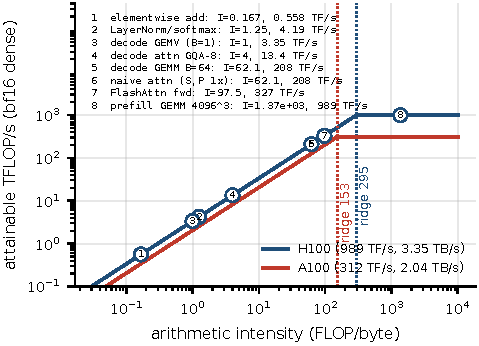
\includegraphics[width=\columnwidth]{fig_roofline}
\caption{A100 与 H100 的 roofline（BF16 稠密，HBM），以及 Transformer 典型算子在 H100 上的位置。
强度由 \texttt{mlsys\_calc.gemm\_intensity} 与配套 FlashAttention IO 模型（$T=4096,d=128$，SRAM 100~KiB）计算。
只有大 GEMM 越过拐点；decode 相关的全部算子位于斜线段，离拐点差 1--2 个数量级。}
\label{fig:roofline}
\end{figure}

roofline 的三个常见误用值得面试时主动指出。第一，$B$ 必须对应某一级存储；对 L2 或 shared memory 也可以画 roofline，
得到的拐点不同（层次化 roofline）。第二，$P_{\text{peak}}$ 必须对应实际使用的计算单元：A100 的非 tensor-core FP32 只有
19.5~TFLOP/s，与 BF16 tensor core 差 16 倍；FlashAttention-2 减少非矩阵乘 FLOPs 的动机正是这一点~\cite{dao2024flashattention2}。
第三，「GPU 利用率 100\%」不是算力打满：\texttt{nvidia-smi} 的 utilization 只表示采样窗口内有 kernel 在运行。

\begin{qa}{为什么「GPU 利用率 100\%」不代表算力打满？应该看什么？}
\ans \texttt{nvidia-smi} 报告的是有 kernel 驻留的时间比例，一个访存受限的逐元素 kernel 同样可以显示 100\%。
应看 Nsight Compute 的 SM 吞吐与 DRAM 吞吐占峰值的比例，或者直接计算 MFU（模型 FLOPs 利用率，第~\ref{sec:kernel} 节）。
DRAM 吞吐接近峰值而 SM 吞吐低，说明受访存限制，下一步是融合或降低精度，而不是调 block size。
\wrong 「100\% 说明已经最优」；或把 HFU（含重计算 FLOPs）当成 MFU 报告。
\end{qa}

\subsection{Amdahl 与 Gustafson 定律}

设程序中可并行部分占比为 $p$，用 $n$ 个处理器时，Amdahl 定律~\cite{amdahl1967validity} 给出固定问题规模下的加速比
\begin{equation}
S_{\text{A}}(n) = \frac{1}{(1-p) + p/n} \xrightarrow{n\to\infty} \frac{1}{1-p}.
\end{equation}
Gustafson~\cite{gustafson1988reevaluating} 指出，实际中问题规模常随资源增长，若并行部分的工作量放大 $n$ 倍，
则 $S_{\text{G}}(n)=(1-p)+pn$。图~\ref{fig:amdahl} 对比了两者：$p=0.95$ 时 8 核只有 5.9 倍，无穷多核也只有 20 倍；
而 Gustafson 视角下加速比随 $n$ 近似线性增长。两者并不矛盾：前者回答「同一个任务能快多少」，
后者回答「同样的时间能做多大的任务」。大模型训练中的弱扩展（增大 global batch）正是 Gustafson 视角，
但它受临界 batch size 的限制，不能无限扩展。

\begin{figure}[!t]
\centering
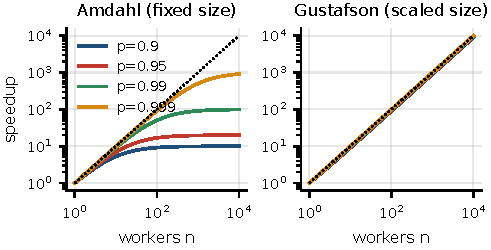
\includegraphics[width=\columnwidth]{fig_amdahl}
\caption{Amdahl（固定规模）与 Gustafson（规模随处理器数增长）加速比，虚线为线性加速。
$p=0.99$ 时 1024 个处理器的 Amdahl 加速比只有 91 倍（\texttt{mlsys\_calc.amdahl\_speedup}）。}
\label{fig:amdahl}
\end{figure}

\begin{qa}{Amdahl 定律在大模型训练里体现在哪里？}
\ans 体现在不随卡数缩小的部分：dataloader 的串行段、优化器步进中的全局梯度范数、日志与 checkpoint、
all-reduce 的延迟项 $2(p-1)\alpha$、流水线气泡，以及负载不均时最慢的 rank。卡数上去之后，这些部分决定 MFU 的上限。
\wrong 「训练是完全数据并行的，没有串行部分」。
\end{qa}

\subsection{Work--span 模型与调度}

把并行计算建模为有向无环图，$T_1$ 为总工作量（work），$T_\infty$ 为关键路径长度（span），并行度为 $T_1/T_\infty$。
Brent 定理~\cite{brent1974parallel} 与贪心调度给出
\begin{equation}
T_P \le \frac{T_1}{P} + T_\infty,
\label{eq:brent}
\end{equation}
Blumofe 与 Leiserson 证明随机 work stealing 在期望意义下达到 $T_1/P+O(T_\infty)$~\cite{blumofe1999scheduling}：
每个线程从自己的双端队列尾部取任务，空闲时随机从别人队列头部「偷」，偷到的往往是大块工作，争抢少。
式~\eqref{eq:brent} 的直接推论是线性加速的条件 $P\ll T_1/T_\infty$。

scan（前缀和）是检验 work--span 思维的标准例子~\cite{blelloch1990prefix,hillis1986data}。Hillis--Steele 算法 span 为 $\log_2 n$，
work 为 $n\log_2 n$；Blelloch 算法 work 为 $2(n-1)$，span 为 $2\log_2 n$。
\lab{CS149 A3}的计数器与公式逐一相等：$n=2^{20}$ 时 Blelloch 做 2.10M 次加法、40 步，Hillis--Steele 做 19.9M 次、20 步；
处理器多于数据时（$n=1000,P=2048$）Hillis--Steele 的 Brent 上界 15 低于 Blelloch 的 21，处理器少时 work 主导，Blelloch 胜出。
GPU 上的工程结论是：大数组用 work-efficient 的 Blelloch，warp 内（32 个元素）用 Hillis--Steele，因为线程本来就空着。

负载均衡是 work--span 的另一面。\lab{CS149 A1}在 Mandelbrot 上比较了三种划分：4 个 worker 时连续块划分 2.93 倍、
交错行 3.93 倍、动态分块 3.76 倍；8 块静态划分时中间块耗时 0.233~s 而边缘块只有 0.063~s。
同一实验的第一版曾测出 8 个 worker 21 倍的「超线性加速」，原因是按 worker 数切块改变了 numpy 中间数组的缓存行为，
基线不公平——这是一个很好的面试故事：超线性加速首先怀疑基线。

\begin{qa}{静态分配和动态分配怎么选？work stealing 为什么好？}
\ans 任务代价可预测且均匀时用静态划分（零调度开销）；不可预测时用动态。集中式队列会成为争抢热点，work stealing 让每个线程
优先处理本地任务，只有空闲时才偷，并且偷队列另一端的大块任务，满足 $T_P\le T_1/P+O(T_\infty)$。
\wrong 「动态一定比静态好」——细粒度任务的入队出队开销可能比任务本身还大。
\end{qa}

\subsection{Little 定律与服务容量}

对任何稳态排队系统，Little 定律~\cite{little1961proof} 给出 $L=\lambda W$：系统中平均请求数等于到达率乘以平均停留时间。
它不依赖到达分布与服务分布，因此是推理服务容量规划的第一公式。设平均输出 500 token、每 token 时延（TPOT）30~ms、
首 token 时延（TTFT）0.5~s，则 $W\approx 15.5$~s；若 KV 预算只允许 64 条并发，则 $\lambda_{\max}\approx 64/15.5\approx 4.1$~req/s。
同样的定律也解释了 GPU 的延迟隐藏：要维持带宽 $\mathrm{BW}$、访存延迟 $\ell$，在途字节数必须达到 $\mathrm{BW}\cdot\ell$，
这是 occupancy 与异步拷贝存在的理由（第~\ref{sec:hw} 节）。

\begin{est}{H100 需要多少在途字节才能吃满 HBM？}
取 HBM 带宽 3.35~TB/s、访存延迟约 500 个周期（约 0.3~\textmu s，附录表~\ref{tab:hw} 的数量级）。
由 Little 定律，在途字节 $\approx 3.35\times10^{12}\times 3\times10^{-7}\approx 1$~MB；分到 132 个 SM，每个 SM 约 7.6~KB 在途。
若每个线程每次发起 16 字节的向量加载，每个 SM 需要约 480 个线程同时有访存在途。这就是为什么访存受限 kernel
需要较高 occupancy 或者 TMA/\texttt{cp.async} 这类异步批量拷贝。
\end{est}

\subsection{I/O 复杂度下界}

Hong 与 Kung 的红蓝卵石游戏~\cite{hong1981io} 证明，快速存储容量为 $M$ 时，$n\times n$ 矩阵乘至少需要
$\Omega(n^3/\sqrt{M})$ 次慢速存储访问。这个下界把「分块」从技巧变成了必然：任何达到下界的算法都必须让每个
加载进快存的元素被复用 $\Theta(\sqrt{M})$ 次。FlashAttention 论文给出了 attention 的类似下界
$\Omega(T^2d^2/M)$~\cite{dao2022flashattention}，我们在第~\ref{sec:kernel} 节会看到，这个下界在 $d^2/M$ 不太小时
意味着 HBM 流量仍是 $T$ 的二次函数。

\begin{keypts}
\begin{itemize}
\item roofline：$t\ge\max(F/P,B/\mathrm{BW})$；H100 拐点 295、A100 拐点 153~FLOP/B，必须说明对应哪个计算单元与哪级存储。
\item Amdahl 给固定规模的上限，Gustafson 给扩展规模的视角；训练中的串行项包括通信延迟与流水线气泡。
\item work--span：$T_P\le T_1/P+T_\infty$；scan 的两种算法分别优化 span 与 work。
\item Little 定律 $L=\lambda W$ 同时适用于服务容量和 GPU 延迟隐藏。
\end{itemize}
\end{keypts}

\begin{research}
\begin{itemize}
\item roofline 假设计算与访存完全重叠。一个好问题是：对于 FlashAttention 这类「矩阵乘 + 逐元素」交替的 kernel，
重叠不完美导致的偏差有多大？可以用 Nsight 的指令级采样把时间分解为 tensor core 忙、等待 TMA、等待 softmax 三部分。
\item 设计实验验证 Little 定律在 LLM 服务里的适用边界：在 continuous batching 下，停留时间 $W$ 本身依赖并发 $L$
（batch 越大每步越慢），系统是否仍存在唯一稳态？
\end{itemize}
\end{research}
